%File: main.tex
\documentclass[letterpaper]{article} % DO NOT CHANGE THIS
\usepackage[submission]{aaai2026}  % DO NOT CHANGE THIS
\usepackage{times}  % DO NOT CHANGE THIS
\usepackage{helvet}  % DO NOT CHANGE THIS
\usepackage{courier}  % DO NOT CHANGE THIS
\usepackage[hyphens]{url}  % DO NOT CHANGE THIS
\usepackage{graphicx} % DO NOT CHANGE THIS
\urlstyle{rm} % DO NOT CHANGE THIS
\def\UrlFont{\rm}  % DO NOT CHANGE THIS
\usepackage{natbib}  % DO NOT CHANGE THIS AND DO NOT ADD ANY OPTIONS TO IT
\usepackage{caption} % DO NOT CHANGE THIS AND DO NOT ADD ANY OPTIONS TO IT
\frenchspacing  % DO NOT CHANGE THIS
\setlength{\pdfpagewidth}{8.5in} % DO NOT CHANGE THIS
\setlength{\pdfpageheight}{11in} % DO NOT CHANGE THIS

\usepackage{amsmath}
\usepackage{booktabs}

\pdfinfo{
/TemplateVersion (2026.1)
}

\setcounter{secnumdepth}{2}

% Title
\title{Auditing Engagement Incentives in the Kidfluencer Ecosystem: A Multimodal Weak Supervision Approach}
\author{
    Anonymous Submission
}
\affiliations{
}

\begin{document}

\maketitle

\begin{abstract}
The rapid rise of ``kidfluencers'' on YouTube has raised profound ethical concerns regarding child digital labor and exploitation. While emerging legislation attempts to regulate this ecosystem, empirical evidence on the relationship between child exploitation and engagement metrics remains scarce due to the challenge of operationalizing and scaling exploitation measurements. This study presents a multimodal AI audit of 5,051 videos across 79 kidfluencer channels, utilizing a weak supervision approach to detect exploitation signals without requiring large-scale manually labeled ground truth. We aggregate noisy labeling functions---including LLM-based classification of titles and GPT-4 Vision analysis of thumbnails and descriptions across six literature-grounded dimensions---to assign a probabilistic exploitation score to each video.

Our findings reveal a highly significant \textbf{engagement premium associated with performative labor, emotional bait, and privacy violations}. Overall exploitation scores correlate significantly with view counts (Spearman $\rho = 0.328$, $p < 10^{-126}$). Mixed-effects regression, controlling for channel-level variation, demonstrates that a one-unit increase in exploitation score is associated with a 4.8$\times$ increase in views ($p < 0.001$). Within-channel analyses show that performative content is associated with a median view boost of $+42.0\%$ (FDR-corrected $p<0.001$). These effects hold in robustness checks comparing videos published within the same year ($p=0.006$). Conversely, we find that explicit commercial content (product placement) exhibits a significant \emph{negative} premium ($-32.5\%$, $p=0.012$), suggesting that the platform ecosystem rewards the commodification of the child's identity and labor rather than traditional advertising. These findings challenge policy frameworks focused solely on financial trusts, demonstrating that engagement metrics systematically reward the intensive, performative labor of children.
\end{abstract}

\section{Introduction}

The commercialization of childhood through digital platforms has created a lucrative ``kidfluencer'' economy in which children are featured in YouTube videos---unboxing toys, participating in challenges, performing scripted roleplay, and documenting their daily lives \citep{clark2025child}. This phenomenon has sparked intense debate regarding the ethics of child digital labor, the psychological impact of public exposure, and the blurring of lines between play and work, often termed ``playbour'' \citep{abidin2015micromicrocelebrity}.

Recent legislative efforts, such as the Illinois PA 103-0556 (2024) \citep{illinois2024}, aim to protect child creators by mandating financial trusts and limiting working hours. However, these regulations treat kidfluencing as a traditional labor market, often failing to address how platform ecosystems actively shape content creation \citep{unicef2025}. A fundamental question remains: \textbf{How do engagement metrics associate with specific dimensions of child exploitation?}

Previous research on the kidfluencer ecosystem has largely relied on qualitative content analysis or small-scale manual coding \citep{divon2025children,anderson2025growing}. While valuable, these approaches cannot scale to audit the massive volume of content generated. Conversely, purely computational approaches often struggle to operationalize complex, nuanced concepts like ``exploitation'' or ``performativity'' without expensive, large-scale human annotation. Furthermore, prior audits of platform algorithms \citep{huszar2022algorithmic,haroon2023auditing} have often focused on political content rather than child safety \citep{papadamou2020disturbed}.

This study bridges this gap by deploying a \textbf{multimodal weak supervision pipeline} to conduct a large-scale observational audit. We ground our definition of exploitation in the UN Convention on the Rights of the Child (UNCRC) and recent theoretical frameworks \citep{clark2025child,divon2025children}, operationalizing six specific dimensions: performative labor, emotional bait, narrative conflict, challenge formats, commercial content, and privacy violations.

Crucially, because we rely on observational data via the YouTube API, we cannot directly observe the recommendation algorithm's internal scoring \citep{bouchaud2024auditing,rieder2018ranking}. Instead, we measure the \textbf{engagement premium}---the association between exploitative content dimensions and view counts---which serves as a proxy for the incentive structures shaping creator behavior.

Our core research questions are:
\begin{itemize}
    \item \textbf{RQ1:} Can a weak supervision framework effectively synthesize multimodal signals (text, LLM classifications, and computer vision) to measure kidfluencer exploitation at scale?
    \item \textbf{RQ2:} Are specific dimensions of exploitation (e.g., performative labor vs.\ commercial content) associated with higher view counts (an ``engagement premium'')?
    \item \textbf{RQ3:} Does this engagement premium persist \emph{within} channels and when controlling for video age, indicating a structural correlation rather than merely a channel-popularity effect?
\end{itemize}

\section{Related Work}

\subsection{The Kidfluencer Economy and Exploitation Frameworks}

The kidfluencer economy relies on the continuous documentation of children's private lives and their participation in scripted entertainment. Clark and Jno-Charles \citep{clark2025child} propose analyzing this phenomenon through the lens of the UNCRC, identifying fundamental threats to children's rights: economic exploitation, exposure to harm, and restriction of authentic expression. Divon et al.\ \citep{divon2025children} further describe how children are transformed into ``concealed commodities'' through practices like transactional play.

Other literature highlights the privacy risks of ``sharenting'' \citep{steinberg2017sharenting,kopecky2020sharenting}, where parents overshare children's lives online, potentially leading to emotional neglect \citep{keskin2023sharenting}. In extreme cases, such as the ``Elsagate'' phenomenon, platforms have struggled to moderate inappropriate content targeting toddlers \citep{papadamou2020disturbed,bridle2017something,tahir2019bringing}. Building on these frameworks, we operationalize exploitation not merely as overt abuse, but as the intensive, performative labor required to maintain engagement.

\subsection{Algorithmic Auditing and Engagement Metrics}

Algorithmic auditing investigates platform behavior without direct access to proprietary code \citep{sandvig2014auditing,metaxa2021auditing}. Studies have audited YouTube and Twitter for political radicalization and amplification \citep{ribeiro2020auditing,huszar2022algorithmic,haroon2023auditing,hussein2020measuring}, often using sock puppets \citep{habib2025auditing} or observational engagement data \citep{bouchaud2024auditing}. Since direct recommendation rates are hidden, researchers often use engagement metrics (views, likes) as proxies for algorithmic reach \citep{covington2016deep,zhou2010impact,rieder2018ranking}. We adopt this observational approach, focusing on the ``engagement premium'' associated with specific content types.

\subsection{Weak Supervision and LLM Content Analysis}

Traditional machine learning requires massive labeled datasets, which are difficult to obtain for subjective concepts. Weak supervision frameworks like Snorkel \citep{ratner2017snorkel,ratner2016data,bach2019snorkel} allow researchers to encode domain knowledge as noisy heuristic rules (Labeling Functions) to generate probabilistic labels \citep{johnson2022survey}. Recently, Large Language Models (LLMs) and Vision-Language Models (VLMs) have shown promise in zero-shot content moderation and annotation \citep{ma2023adapting,gilardi2023chatgpt,tornberg2024chatgpt}. We combine LLMs and VLMs within a weak supervision framework to scale our exploitation analysis across text and visual modalities.

\section{Methodology}

\subsection{Data Collection and Sampling}

We collected metadata for 58,965 videos from 79 family and kidfluencer YouTube channels using the YouTube Data API. Channels were selected based on prior literature and popular influencer lists, covering a spectrum of channel sizes and target audiences. The selected 79 channels represent a diverse cross-section of the kidfluencer ecosystem: 9 small channels ($<$50K median views), 31 medium (50K--500K), 26 large (500K--5M), and 13 very large ($>$5M median views), with an overall median of approximately 445,000 views per video. All channels are primarily English-language family vlog or kidfluencer channels featuring real children; animated channels were strictly excluded.

To manage computational costs while maintaining representativeness, we employed a stratified sampling strategy. For each of the 79 channels, we stratified videos into terciles based on view counts (high, medium, low) and randomly sampled up to 20 videos per tercile, resulting in a final stratified sample of 5,051 videos with valid view counts. We retrieved the title, description, thumbnail image, and publication date for each sampled video.

\subsection{Exploitation Dimensions}

Based on Clark and Jno-Charles \citep{clark2025child} and Divon et al.\ \citep{divon2025children}, we defined six exploitation dimensions:
\begin{enumerate}
    \item \textbf{Performative Labor:} Child performing scripted/planned content for the camera.
    \item \textbf{Emotional Bait:} Using the child's exaggerated emotions for clickbait.
    \item \textbf{Narrative Conflict:} Manufactured drama or conflict involving the child.
    \item \textbf{Challenge Format:} High-effort competition formats requiring extended labor.
    \item \textbf{Commercial Content:} Child used explicitly for product placement/unboxing.
    \item \textbf{Privacy Violation:} Exposure of the child's private, vulnerable, or medical moments.
\end{enumerate}

\subsection{Multimodal Weak Supervision Pipeline}

We implemented a multimodal weak supervision pipeline utilizing two primary signal sources, aggregated using a weighted combination:

\textbf{LLM Text Classification (Weight = 0.33):} We deployed GPT-4.1-mini to classify video titles along the six dimensions. This provided a binary classification ($0$ or $1$) for each dimension based solely on textual metadata.

\textbf{VLM Multimodal Classification (Weight = 0.67):} We deployed the GPT-4.1-mini Vision API to analyze the combination of the video's title, thumbnail image, and description. The VLM provided a continuous probability score ($[0, 1]$) for each dimension.

The VLM and LLM signals were aggregated using a weighted average. We assigned a weight of 0.67 to the VLM and 0.33 to the LLM, reflecting the structural prior that the VLM analyzes a richer multimodal context (title, thumbnail, and description) compared to the LLM's text-only analysis (title). Sensitivity analyses confirmed that the highly significant correlation between the resulting exploitation score and view counts ($p < 10^{-6}$) is robust across all possible weighting schemes, including relying solely on the VLM or the LLM (see Section~\ref{sec:robustness}).

Validation on a subset of 50 human-annotated videos demonstrated that the combined multimodal pipeline achieved strong discriminative ability, with an AUC-ROC of $0.795$ and a significant rank correlation with human judgments (Spearman $\rho = 0.455$, $p=0.002$). For the most prevalent dimension, performative labor, the pipeline performed exceptionally well (AUC-ROC $= 0.915$, $\kappa = 0.650$). Validation was conducted by a single trained annotator using the definitions in Section~3.2; future work should employ multiple independent annotators to establish inter-rater reliability.

The pipeline computed a combined score for each dimension, and an \textbf{Overall Exploitation Score} $\in [0, 1]$ for each video.

\section{Results}

\subsection{Pipeline Performance and Dimension Prevalence}

The multimodal pipeline successfully processed 4,673 videos (92.5\% coverage for vision analysis). Overall, 19.7\% of the sampled videos ($n=997$) were classified as exploitative (score $\ge 0.5$).

\begin{figure}[t]
\centering
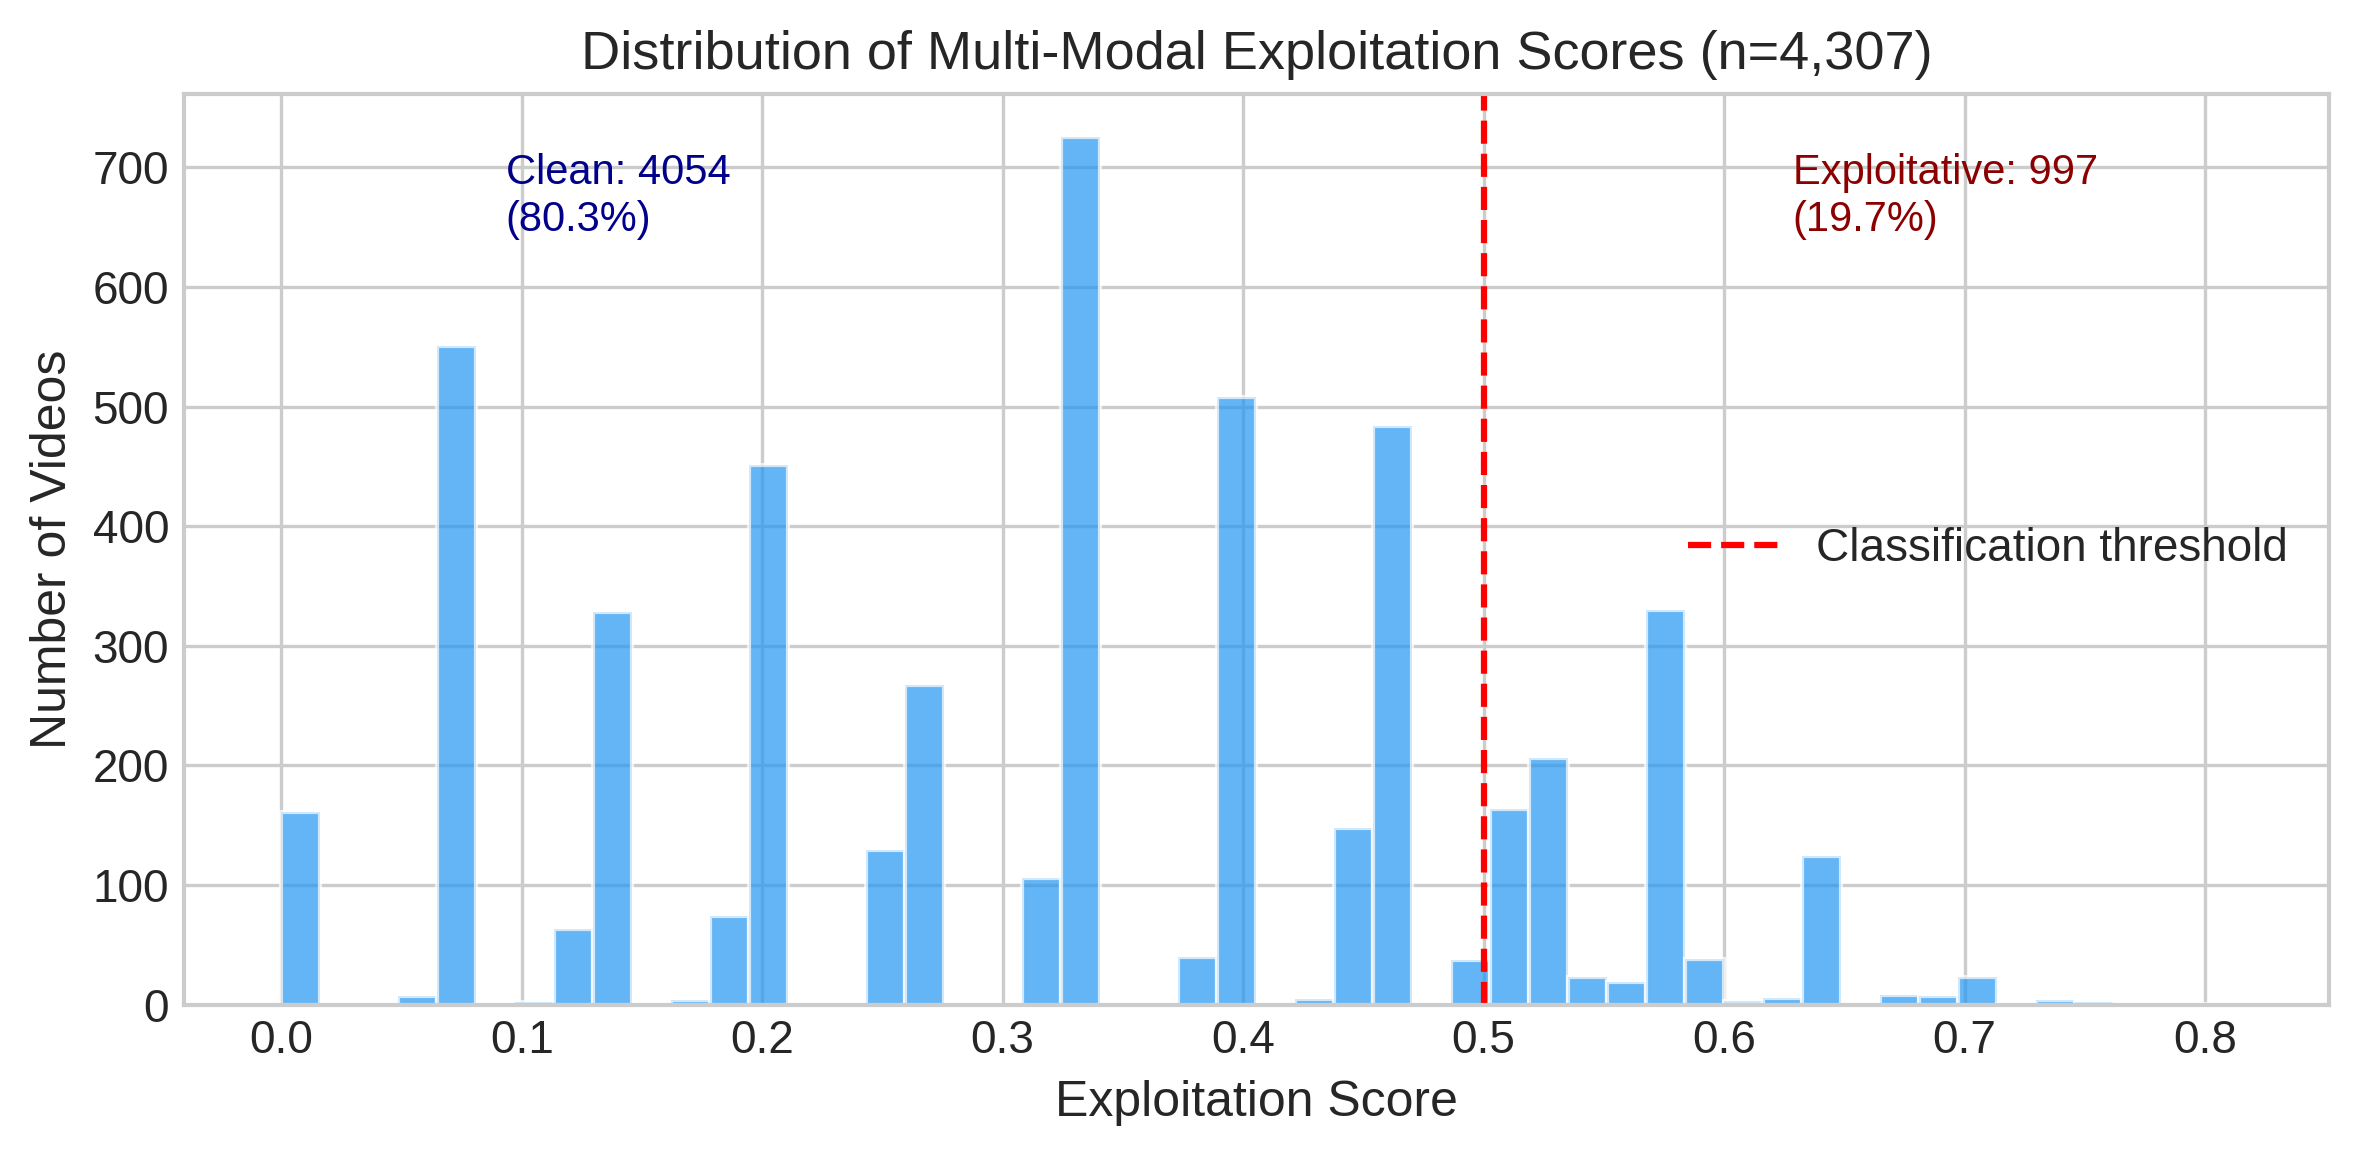
\includegraphics[width=\columnwidth]{fig1_score_distribution.png}
\caption{Distribution of the probabilistic exploitation score generated by the multimodal weak supervision model.}
\label{fig:score_dist}
\end{figure}

Performative labor was the most prevalent dimension (detected in 60.5\% of videos by the VLM), followed by emotional bait (45.0\%), narrative conflict (26.8\%), challenge formats (19.2\%), commercial content (18.5\%), and privacy violations (4.2\%).

\subsection{The Engagement Premium (RQ2 \& RQ3)}

We found a highly significant positive correlation between a video's overall Exploitation Score and its view count (Spearman $\rho = 0.328$, $p < 10^{-126}$).

To determine if this association is a structural platform correlation rather than merely an artifact of highly exploitative channels being more popular overall, we conducted two primary analyses: mixed-effects regression and within-channel pairwise comparisons.

\subsubsection{Mixed-Effects Regression.}

We fit a mixed-effects linear regression model predicting $\log_{10}(\text{views})$ from the overall exploitation score, including random intercepts for each of the 79 channels to control for baseline channel popularity.

The model revealed a massive, highly significant effect: a one-unit increase in the exploitation score is associated with a $0.681$ increase in $\log_{10}(\text{views})$ ($\beta = 0.681$, $SE = 0.054$, $z = 12.61$, $p < 0.001$). This translates to approximately a \textbf{4.8$\times$ increase in raw view counts} ($10^{0.681} \approx 4.8$).

We then fit a second mixed-effects model using the six individual dimensions as fixed effects. When controlling for all dimensions simultaneously, \textbf{performative labor} ($\beta = 0.291$, $p < 0.001$), \textbf{privacy violations} ($\beta = 0.316$, $p < 0.001$), and \textbf{emotional bait} ($\beta = 0.205$, $p < 0.001$) remained highly significant predictors of increased viewership. Narrative conflict, challenge formats, and commercial content lost statistical significance in the joint model, suggesting their effects may be partially mediated by correlation with the primary three dimensions.

\subsubsection{Within-Channel Pairwise Comparisons.}

For each dimension, we compared the median views of videos exhibiting that dimension against videos from the \emph{same channel} lacking it. To account for multiple comparisons, we applied False Discovery Rate (FDR) correction using the Benjamini-Hochberg procedure.

\begin{figure}[t]
\centering

\includegraphics[width=\columnwidth]{fig2_dimension_premiums.png}
\caption{Mean within-channel view boost by exploitation dimension (FDR-corrected). Error bars represent 95\% confidence intervals.}
\label{fig:premiums}
\end{figure}

The results reveal a clear engagement premium structure across 54 channels with sufficient data:
\begin{itemize}
    \item \textbf{Performative Labor} is associated with a mean within-channel log-premium of $+0.354$ (Cohen's $d = 0.613$, FDR $p<0.001$).
    \item \textbf{Privacy Violations} are associated with a mean log-premium of $+0.401$ (FDR $p=0.012$).
    \item \textbf{Emotional Bait} is associated with a mean log-premium of $+0.281$ (FDR $p=0.001$).
    \item \textbf{Challenge Formats} and \textbf{Narrative Conflict} also showed significant positive premiums (FDR $p < 0.05$).
\end{itemize}

Crucially, \textbf{Commercial Content} exhibited a significant \textbf{negative} premium (mean log-premium $-0.325$, FDR $p=0.012$). Videos featuring explicit product placements or unboxing received systematically \emph{fewer} views than non-commercial videos on the same channel.

\begin{figure}[t]
\centering

\includegraphics[width=\columnwidth]{fig5_emotional_vs_commercial.png}
\caption{Contrasting effects: Emotional exploitation dimensions show positive engagement premiums while commercial content shows a negative premium.}
\label{fig:contrast}
\end{figure}

\subsection{Robustness Checks}
\label{sec:robustness}

To ensure our findings were not merely artifacts of video age (older videos accumulating more views), we conducted a \textbf{same-year within-channel comparison}. By matching exploitative and non-exploitative videos published by the same channel in the same year (37 channel-year groups), we found the engagement premium holds robustly: high-exploitation videos received a mean log-premium of $+0.404$ over their same-year, same-channel counterparts (Wilcoxon $p=0.006$).

\begin{figure}[t]
\centering
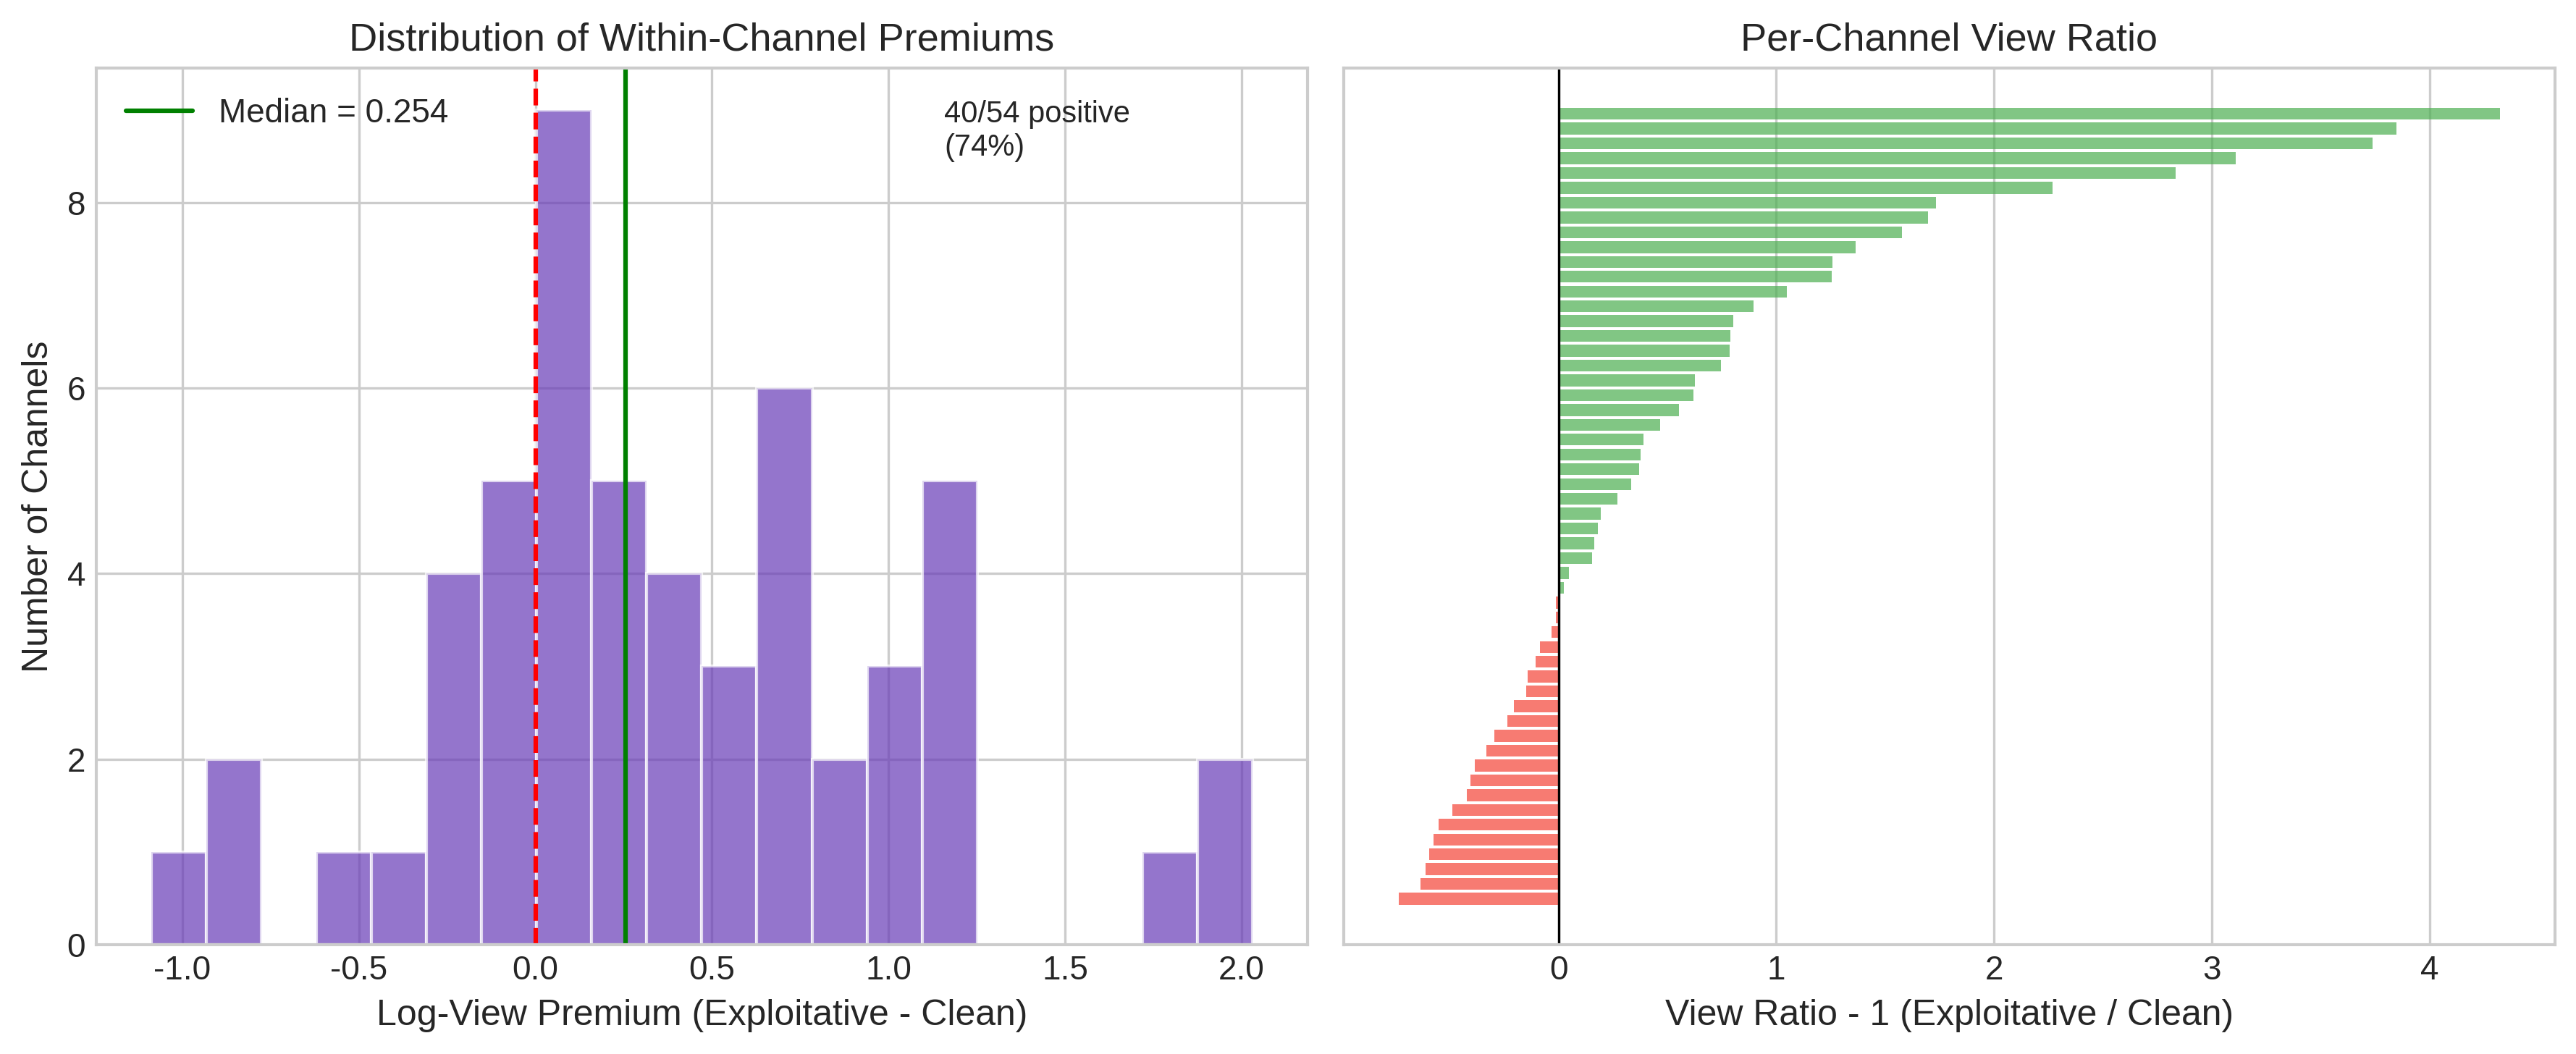
\includegraphics[width=\columnwidth]{fig4_channel_premiums.png}
\caption{Distribution of overall within-channel premiums. 74.1\% of channels exhibit a positive premium for exploitative content.}
\label{fig:channel_dist}
\end{figure}

Additionally, we conducted a weight sensitivity analysis. The Spearman correlation between exploitation score and view counts remained highly significant ($p < 10^{-6}$) across all possible VLM/LLM weight combinations tested (from 100\% VLM to 100\% LLM), confirming that our findings are not an artifact of the specific weighting scheme chosen.

\section{Discussion}

\subsection{The ``Performativity Premium'' vs.\ The Commercial Penalty}

Our findings provide large-scale empirical evidence for a ``performativity premium'' in the kidfluencer ecosystem. Engagement metrics are systematically associated with content that requires children to engage in intensive, performative labor (scripted conflict, emotional bait) over organic family documentation.

Interestingly, traditional commercial content suffers a penalty. This suggests a fundamental shift in the kidfluencer economy: the most successful strategy is not to use the child to sell a physical toy, but to make the child's labor, emotions, and manufactured drama the product itself. This aligns with Divon et al.'s \citep{divon2025children} concept of ``transactional childhood.'' Audiences appear to reject overt advertising but heavily reward the commodification of the child's identity and emotional vulnerability.

\subsection{Methodological Contributions}

This study demonstrates the efficacy of multimodal weak supervision for large-scale observational auditing. By combining LLM text analysis and VLM visual analysis, we successfully scaled the operationalization of complex ethical concepts without requiring massive manual ground truth. The strong discriminative ability (AUC-ROC $= 0.795$) and significant rank correlation ($\rho = 0.455$) between our multimodal pipeline and human annotations offer a blueprint for future audits of subjective content moderation issues.

\subsection{Limitations and Future Work}

This study has several limitations. First, our validation relied on a single trained annotator ($n=50$). While our pipeline achieved strong discriminative ability against this baseline, future research must employ multiple independent annotators to establish rigorous inter-rater reliability, particularly given the subjective nature of dimensions like ``emotional bait.'' As noted during annotation, distinguishing between genuine family vlogs and manufactured ``staged drama'' often requires contextual understanding beyond what thumbnails and descriptions provide.

Second, our analysis relies on observational data. We measure \emph{engagement metrics} (views), which are proxies for algorithmic reach, but we cannot claim a direct causal link to YouTube's internal recommendation weights \citep{rieder2018ranking}. The engagement premium we observe may reflect audience preferences, algorithmic amplification, or both.

Third, our VLM classification primarily analyzed video titles, thumbnails, and descriptions; future work should incorporate full video transcripts and duration data to capture intra-video dynamics. Finally, our sample is limited to English-language channels; cross-cultural analyses may reveal different exploitation patterns and engagement dynamics.

\section{Ethics Statement}

This research utilizes publicly available, observational data from YouTube via the official API. The study was deemed IRB-exempt as it involves no direct interaction with human subjects or minors, and analyzes public figures in the digital economy. We report aggregate statistics to protect the privacy of specific children featured in the channels.

\section{Conclusion}

As the kidfluencer economy matures, regulatory focus must expand beyond financial compensation to address the structural forces shaping content creation. Our multimodal audit of 5,051 videos demonstrates that engagement metrics are significantly associated with content featuring child performative labor, privacy violations, and emotional bait, while penalizing overt commercial content. By highlighting this ``performativity premium,'' this study underscores the need for platform-level interventions that disincentivize the commodification of child labor and stress.

\bibliography{references}
\bibliographystyle{aaai2026}

\end{document}
